\documentclass[aspectratio=169]{beamer}
\usepackage[utf8]{inputenc}
\usepackage{lmodern}
\usepackage[T1]{fontenc}
\usepackage{listings}
\usepackage{tikz}
\usetikzlibrary{arrows.meta, positioning, shapes.geometric, calc}

% Set path to find the theme
\makeatletter
\def\input@path{{../BeamerTemplate/theme/}}
\makeatother

\usetheme{CleanEasy}
\input{../BeamerTemplate/configs/configs}

% Listings configuration
\lstset{
    basicstyle=\ttfamily\footnotesize,
    keywordstyle=\color{blue},
    commentstyle=\color{gray},
    stringstyle=\color{red},
    showstringspaces=false,
    breaklines=true,
    frame=single,
    numbers=left,
    numberstyle=\tiny\color{gray}
}

\title{Dynamic Programming}
\subtitle{Optimize Recursive Solutions by Reusing Subproblem Results}
\author{Minseok Jeon}
\institute{DGIST}
\date{\today}

\begin{document}

\begin{frame}
  \titlepage
\end{frame}

\begin{frame}{Table of Contents}
  \tableofcontents
\end{frame}

\section{Introduction}

\begin{frame}{What is Dynamic Programming?}
  \textbf{Dynamic Programming (DP)}: An optimization technique for recursive problems

  \vspace{0.5cm}

  \textbf{Core Idea}:
  \begin{itemize}
    \item Break problem into overlapping subproblems
    \item Solve each subproblem once
    \item Store results to avoid recomputation
    \item Build solution from cached subproblem results
  \end{itemize}

  \vspace{0.5cm}

  \textbf{Key Difference from Divide-and-Conquer}:
  \begin{itemize}
    \item \textbf{D\&C}: Subproblems are independent (merge sort, quicksort)
    \item \textbf{DP}: Subproblems overlap (fibonacci, shortest path)
  \end{itemize}
\end{frame}

\begin{frame}{When to Use Dynamic Programming}
  \textbf{Two Required Properties}:

  \vspace{0.3cm}

  \begin{enumerate}
    \item \textbf{Overlapping Subproblems}
    \begin{itemize}
      \item Same subproblems solved multiple times in naive recursion
      \item Caching results provides significant speedup
    \end{itemize}

    \vspace{0.3cm}

    \item \textbf{Optimal Substructure}
    \begin{itemize}
      \item Optimal solution contains optimal solutions to subproblems
      \item Can build global optimum from local optima
    \end{itemize}
  \end{enumerate}

  \vspace{0.5cm}

  \textbf{Additional Requirement}:
  \begin{itemize}
    \item Must be able to define recursive relation between states
  \end{itemize}
\end{frame}

\section{Overlapping Subproblems and Optimal Substructure}

\begin{frame}{Overlapping Subproblems: Fibonacci Example}
  \textbf{Problem}: Compute $n$-th Fibonacci number

  \vspace{0.3cm}

  \begin{center}
  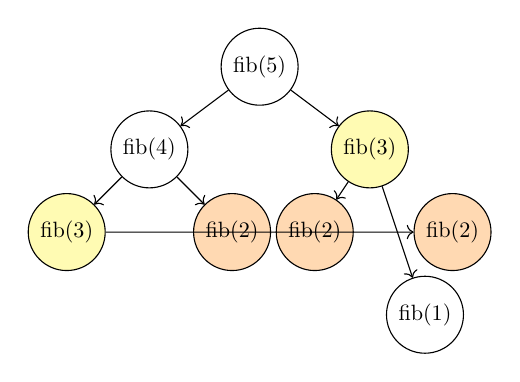
\begin{tikzpicture}[scale=0.7, every node/.style={scale=0.8}]
    \node[circle, draw] (f5) at (0,0) {fib(5)};
    \node[circle, draw] (f4) at (-2,-1.5) {fib(4)};
    \node[circle, draw, fill=yellow!30] (f3a) at (2,-1.5) {fib(3)};
    \node[circle, draw, fill=yellow!30] (f3b) at (-3.5,-3) {fib(3)};
    \node[circle, draw, fill=orange!30] (f2a) at (-0.5,-3) {fib(2)};
    \node[circle, draw, fill=orange!30] (f2b) at (1,-3) {fib(2)};
    \node[circle, draw, fill=orange!30] (f2c) at (3.5,-3) {fib(2)};
    \node[circle, draw] (f1a) at (3,-4.5) {fib(1)};

    \draw[->] (f5) -- (f4);
    \draw[->] (f5) -- (f3a);
    \draw[->] (f4) -- (f3b);
    \draw[->] (f4) -- (f2a);
    \draw[->] (f3a) -- (f2b);
    \draw[->] (f3a) -- (f1a);
    \draw[->] (f3b) -- (f2c);
  \end{tikzpicture}
  \end{center}

  \textbf{Observation}:
  \begin{itemize}
    \item fib(3) computed 2 times (yellow)
    \item fib(2) computed 3 times (orange)
    \item \textbf{Exponential time}: $O(2^n)$ without caching
  \end{itemize}
\end{frame}

\begin{frame}[fragile]{Naive Recursion vs Memoization}
\begin{columns}
\begin{column}{0.48\textwidth}
\textbf{Naive Recursion: $O(2^n)$}
\begin{lstlisting}[language=Python, basicstyle=\ttfamily\tiny]
def fib(n):
    if n <= 1:
        return n
    return fib(n-1) + fib(n-2)

# fib(40) takes seconds!
\end{lstlisting}
\end{column}

\begin{column}{0.48\textwidth}
\textbf{With Memoization: $O(n)$}
\begin{lstlisting}[language=Python, basicstyle=\ttfamily\tiny]
def fib_memo(n, memo={}):
    if n in memo:
        return memo[n]
    if n <= 1:
        return n
    memo[n] = fib_memo(n-1, memo) + \
              fib_memo(n-2, memo)
    return memo[n]

# fib_memo(40) instant!
\end{lstlisting}
\end{column}
\end{columns}

\vspace{0.5cm}

\textbf{Key Insight}: Cache results to avoid recomputation
\begin{itemize}
  \item Each subproblem solved exactly once
  \item Lookup takes $O(1)$ time
  \item Total time: $O(n)$ instead of $O(2^n)$
\end{itemize}
\end{frame}

\begin{frame}{Optimal Substructure}
  \textbf{Definition}: Optimal solution contains optimal solutions to subproblems

  \vspace{0.5cm}

  \textbf{Example 1: Shortest Path} $\checkmark$
  \begin{itemize}
    \item If shortest path $A \to C$ goes through $B$
    \item Then $A \to B$ and $B \to C$ must also be shortest paths
    \item Can build optimal solution from optimal subproblems
  \end{itemize}

  \vspace{0.5cm}

  \textbf{Counter-example: Longest Simple Path} $\times$
  \begin{itemize}
    \item Longest path $A \to C$ through $B$
    \item Does \textbf{NOT} guarantee $A \to B$ and $B \to C$ are longest
    \item Why? Cannot revisit nodes (constraint breaks substructure)
    \item This problem is NP-hard!
  \end{itemize}
\end{frame}

\begin{frame}{Problem Classification}
  \begin{center}
  \begin{tabular}{|l|c|c|c|}
    \hline
    \textbf{Problem} & \textbf{Overlapping?} & \textbf{Optimal Substructure?} & \textbf{DP?} \\
    \hline
    Fibonacci & Yes & Yes & $\checkmark$ \\
    Shortest path & Yes & Yes & $\checkmark$ \\
    LIS & Yes & Yes & $\checkmark$ \\
    Knapsack & Yes & Yes & $\checkmark$ \\
    \hline
    Merge sort & No & Yes & $\times$ (D\&C) \\
    Longest simple path & Yes & No & $\times$ (NP-hard) \\
    \hline
  \end{tabular}
  \end{center}

  \vspace{0.5cm}

  \textbf{When to use DP}:
  \begin{itemize}
    \item $\checkmark$ Problem has overlapping subproblems
    \item $\checkmark$ Problem has optimal substructure
    \item $\checkmark$ Can define recursive relation
    \item $\times$ Subproblems independent → use divide-and-conquer
    \item $\times$ No optimal substructure → greedy or other approach
  \end{itemize}
\end{frame}

\section{Top-down (Memoization) vs Bottom-up}

\begin{frame}{Two Approaches to Dynamic Programming}
  \begin{columns}
  \begin{column}{0.48\textwidth}
    \textbf{Top-down (Memoization)}
    \begin{itemize}
      \item Start from original problem
      \item Recurse down to base cases
      \item Cache results along the way
      \item Natural recursive thinking
    \end{itemize}

    \vspace{0.3cm}

    \begin{center}
    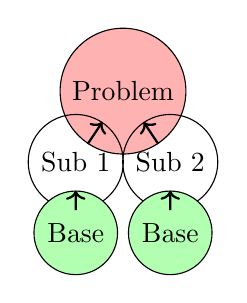
\begin{tikzpicture}[scale=0.6]
      \node[circle, draw, fill=red!30] (n) at (0,0) {Problem};
      \node[circle, draw] (n1) at (-1,-1.5) {Sub 1};
      \node[circle, draw] (n2) at (1,-1.5) {Sub 2};
      \node[circle, draw, fill=green!30] (b1) at (-1,-3) {Base};
      \node[circle, draw, fill=green!30] (b2) at (1,-3) {Base};

      \draw[->, thick] (n) -- (n1);
      \draw[->, thick] (n) -- (n2);
      \draw[->, thick] (n1) -- (b1);
      \draw[->, thick] (n2) -- (b2);
    \end{tikzpicture}
    \end{center}
  \end{column}

  \begin{column}{0.48\textwidth}
    \textbf{Bottom-up (Tabulation)}
    \begin{itemize}
      \item Start from base cases
      \item Build up iteratively
      \item Fill table in correct order
      \item No recursion overhead
    \end{itemize}

    \vspace{0.3cm}

    \begin{center}
    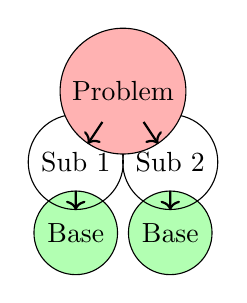
\begin{tikzpicture}[scale=0.6]
      \node[circle, draw, fill=green!30] (b1) at (-1,0) {Base};
      \node[circle, draw, fill=green!30] (b2) at (1,0) {Base};
      \node[circle, draw] (n1) at (-1,1.5) {Sub 1};
      \node[circle, draw] (n2) at (1,1.5) {Sub 2};
      \node[circle, draw, fill=red!30] (n) at (0,3) {Problem};

      \draw[->, thick] (b1) -- (n1);
      \draw[->, thick] (b2) -- (n2);
      \draw[->, thick] (n1) -- (n);
      \draw[->, thick] (n2) -- (n);
    \end{tikzpicture}
    \end{center}
  \end{column}
  \end{columns}
\end{frame}

\begin{frame}[fragile]{Example: Climbing Stairs - Top-down}
  \textbf{Problem}: $n$ stairs, can climb 1 or 2 steps at a time. How many ways to reach top?

  \vspace{0.3cm}

  \textbf{Top-down with Memoization}:
\begin{lstlisting}[language=Python, basicstyle=\ttfamily\footnotesize]
def climb_stairs_memo(n, memo={}):
    # Base cases
    if n <= 2:
        return n

    # Check cache
    if n in memo:
        return memo[n]

    # Recursive relation: ways(n) = ways(n-1) + ways(n-2)
    memo[n] = climb_stairs_memo(n-1, memo) + \
              climb_stairs_memo(n-2, memo)
    return memo[n]
\end{lstlisting}

  \textbf{Time}: $O(n)$ \quad \textbf{Space}: $O(n)$ + recursion stack
\end{frame}

\begin{frame}[fragile]{Example: Climbing Stairs - Bottom-up}
  \textbf{Bottom-up with Tabulation}:
\begin{lstlisting}[language=Python, basicstyle=\ttfamily\footnotesize]
def climb_stairs_dp(n):
    if n <= 2:
        return n

    # DP table
    dp = [0] * (n + 1)
    dp[1] = 1
    dp[2] = 2

    # Fill table bottom-up
    for i in range(3, n + 1):
        dp[i] = dp[i-1] + dp[i-2]

    return dp[n]
\end{lstlisting}

  \textbf{Time}: $O(n)$ \quad \textbf{Space}: $O(n)$

  \vspace{0.3cm}

  \textbf{No recursion overhead, better cache locality}
\end{frame}

\begin{frame}{Comparison: Top-down vs Bottom-up}
  \begin{center}
  \small
  \begin{tabular}{|l|l|l|}
    \hline
    \textbf{Aspect} & \textbf{Top-down} & \textbf{Bottom-up} \\
    \hline
    Direction & Problem $\to$ base cases & Base cases $\to$ problem \\
    Implementation & Recursion + cache & Iteration + table \\
    Subproblems & Only needed & All \\
    Space & $O(n)$ + stack & $O(n)$ \\
    Time overhead & Function calls & None \\
    Intuition & Natural & Requires planning \\
    Space optimization & Harder & Easier \\
    \hline
  \end{tabular}
  \end{center}

  \vspace{0.5cm}

  \textbf{When to choose}:
  \begin{itemize}
    \item \textbf{Top-down}: Recursive solution natural, not all subproblems needed
    \item \textbf{Bottom-up}: Want best performance, need space optimization
  \end{itemize}
\end{frame}

\section{State Definition and Transitions}

\begin{frame}{Designing a DP Solution}
  \textbf{Core of DP}: Properly defining states and transitions

  \vspace{0.5cm}

  \textbf{5-Step Process}:
  \begin{enumerate}
    \item \textbf{Identify what varies}: What parameters change between subproblems?
    \item \textbf{Define DP array}: \texttt{dp[i]}, \texttt{dp[i][j]}, etc.
    \item \textbf{Specify meaning}: What does \texttt{dp[i]} represent?
    \item \textbf{Find recurrence}: How to compute \texttt{dp[i]} from smaller states?
    \item \textbf{Set base cases}: Initial values for smallest subproblems
  \end{enumerate}

  \vspace{0.5cm}

  \textbf{State}: A unique subproblem characterized by parameters

  \textbf{Good state}: Captures all information needed to solve subproblem
\end{frame}

\begin{frame}[fragile]{Example 1: Longest Increasing Subsequence}
  \textbf{Problem}: Find length of longest increasing subsequence in array

  \vspace{0.3cm}

  \textbf{State definition}: \texttt{dp[i]} = length of LIS ending at index $i$

\begin{lstlisting}[language=Python, basicstyle=\ttfamily\tiny]
def length_of_LIS(nums):
    n = len(nums)
    dp = [1] * n  # Base case: each element is LIS of length 1

    # Transition: for each i, check all j < i
    for i in range(1, n):
        for j in range(i):
            if nums[j] < nums[i]:
                dp[i] = max(dp[i], dp[j] + 1)

    return max(dp)  # Answer: maximum among all dp[i]

# Example: [10, 9, 2, 5, 3, 7, 101, 18]
# dp =     [1,  1, 1, 2, 2, 3, 4,   4]
#                      ^        ^
#                   [2,5,7,101] or [2,5,7,18]
\end{lstlisting}

  \textbf{Time}: $O(n^2)$ \quad \textbf{Space}: $O(n)$
\end{frame}

\begin{frame}[fragile]{Example 2: 0/1 Knapsack}
  \textbf{Problem}: $n$ items with weights and values, capacity $W$. Maximize value.

  \vspace{0.3cm}

  \textbf{State}: \texttt{dp[i][w]} = max value using first $i$ items with capacity $w$

\begin{lstlisting}[language=Python, basicstyle=\ttfamily\tiny]
def knapsack(weights, values, W):
    n = len(weights)
    dp = [[0] * (W + 1) for _ in range(n + 1)]

    # Transition
    for i in range(1, n + 1):
        for w in range(W + 1):
            # Don't take item i-1
            dp[i][w] = dp[i-1][w]

            # Take item i-1 (if it fits)
            if weights[i-1] <= w:
                dp[i][w] = max(dp[i][w],
                              dp[i-1][w - weights[i-1]] + values[i-1])

    return dp[n][W]
\end{lstlisting}

  \textbf{Recurrence}: \texttt{dp[i][w] = max(dp[i-1][w], dp[i-1][w-weight[i-1]] + value[i-1])}
\end{frame}

\begin{frame}[fragile]{Example 3: Edit Distance}
  \textbf{Problem}: Min operations to convert word1 to word2 (insert, delete, replace)

  \vspace{0.3cm}

  \textbf{State}: \texttt{dp[i][j]} = min ops to convert \texttt{word1[0..i-1]} to \texttt{word2[0..j-1]}

\begin{lstlisting}[language=Python, basicstyle=\ttfamily\tiny]
def min_distance(word1, word2):
    m, n = len(word1), len(word2)
    dp = [[0] * (n + 1) for _ in range(m + 1)]

    # Base cases
    for i in range(m + 1):
        dp[i][0] = i  # Delete all characters
    for j in range(n + 1):
        dp[0][j] = j  # Insert all characters

    # Transition
    for i in range(1, m + 1):
        for j in range(1, n + 1):
            if word1[i-1] == word2[j-1]:
                dp[i][j] = dp[i-1][j-1]  # No operation needed
            else:
                dp[i][j] = 1 + min(
                    dp[i-1][j],      # Delete from word1
                    dp[i][j-1],      # Insert to word1
                    dp[i-1][j-1]     # Replace
                )
    return dp[m][n]
\end{lstlisting}
\end{frame}

\begin{frame}{Common State Patterns}
  \begin{center}
  \small
  \begin{tabular}{|l|l|l|}
    \hline
    \textbf{Pattern} & \textbf{State} & \textbf{Example Problems} \\
    \hline
    Linear & \texttt{dp[i]} & Fibonacci, climbing stairs \\
    2D grid & \texttt{dp[i][j]} & Unique paths, edit distance \\
    Subsequence & \texttt{dp[i]} ending at $i$ & LIS, max subarray \\
    Knapsack & \texttt{dp[i][w]} & 0/1 knapsack, coin change \\
    Interval & \texttt{dp[i][j]} for [i,j] & Matrix chain mult \\
    State machine & \texttt{dp[i][state]} & Stock trading \\
    \hline
  \end{tabular}
  \end{center}

  \vspace{0.5cm}

  \textbf{Key Insight}: Choose state that:
  \begin{itemize}
    \item Uniquely identifies each subproblem
    \item Contains all necessary information
    \item Allows expressing recurrence relation
    \item Leads to polynomial time/space complexity
  \end{itemize}
\end{frame}

\section{1D/2D DP and Space Optimization}

\begin{frame}[fragile]{Space Optimization: Fibonacci}
  \textbf{Observation}: Only need previous 2 values

\begin{columns}
\begin{column}{0.48\textwidth}
\textbf{1D DP: $O(n)$ space}
\begin{lstlisting}[language=Python, basicstyle=\ttfamily\tiny]
def fib_1d(n):
    dp = [0] * (n + 1)
    dp[1] = 1
    for i in range(2, n + 1):
        dp[i] = dp[i-1] + dp[i-2]
    return dp[n]
\end{lstlisting}
\end{column}

\begin{column}{0.48\textwidth}
\textbf{Optimized: $O(1)$ space}
\begin{lstlisting}[language=Python, basicstyle=\ttfamily\tiny]
def fib_optimized(n):
    if n <= 1:
        return n
    prev2, prev1 = 0, 1
    for i in range(2, n + 1):
        curr = prev1 + prev2
        prev2, prev1 = prev1, curr
    return prev1
\end{lstlisting}
\end{column}
\end{columns}

\vspace{0.5cm}

\textbf{Key Idea}: Keep only what you need
\begin{itemize}
  \item Identify dependencies in recurrence
  \item Store only necessary previous values
  \item Update in correct order
\end{itemize}
\end{frame}

\begin{frame}[fragile]{2D DP Space Optimization: Unique Paths}
  \textbf{Problem}: $m \times n$ grid, count paths from top-left to bottom-right

\begin{columns}
\begin{column}{0.48\textwidth}
\textbf{2D DP: $O(m \times n)$}
\begin{lstlisting}[language=Python, basicstyle=\ttfamily\tiny]
def unique_paths_2d(m, n):
    dp = [[0] * n for _ in range(m)]

    # Base cases
    for i in range(m):
        dp[i][0] = 1
    for j in range(n):
        dp[0][j] = 1

    # Fill table
    for i in range(1, m):
        for j in range(1, n):
            dp[i][j] = dp[i-1][j] + \
                       dp[i][j-1]

    return dp[m-1][n-1]
\end{lstlisting}
\end{column}

\begin{column}{0.48\textwidth}
\textbf{Optimized: $O(n)$}
\begin{lstlisting}[language=Python, basicstyle=\ttfamily\tiny]
def unique_paths_1d(m, n):
    dp = [1] * n  # Only current row

    for i in range(1, m):
        for j in range(1, n):
            dp[j] = dp[j] + dp[j-1]
            # dp[j]: previous row
            # dp[j-1]: current row

    return dp[n-1]
\end{lstlisting}
\end{column}
\end{columns}

\vspace{0.3cm}

\textbf{Observation}: Each row only depends on previous row
\end{frame}

\begin{frame}[fragile]{Rolling Array Technique}
  \textbf{Idea}: Use modulo to reuse array space

\begin{lstlisting}[language=Python, basicstyle=\ttfamily\footnotesize]
def optimized_2d(m, n):
    # Only keep 2 rows in memory
    dp = [[0] * n for _ in range(2)]

    for i in range(m):
        for j in range(n):
            if i == 0 or j == 0:
                dp[i % 2][j] = 1
            else:
                dp[i % 2][j] = dp[(i-1) % 2][j] + dp[i % 2][j-1]

    return dp[(m-1) % 2][n-1]
\end{lstlisting}

  \textbf{When to use}:
  \begin{itemize}
    \item State \texttt{dp[i][j]} only depends on previous row \texttt{dp[i-1][...]}
    \item Reduces space from $O(m \times n)$ to $O(2 \times n)$ or $O(n)$
  \end{itemize}
\end{frame}

\begin{frame}[fragile]{State Compression with Bitmasks}
  \textbf{Use case}: Small state space (e.g., subsets of $n$ items)

  \vspace{0.3cm}

  \textbf{Example: Traveling Salesman Problem}
\begin{lstlisting}[language=Python, basicstyle=\ttfamily\tiny]
def tsp(dist):
    n = len(dist)
    # dp[mask][i] = min cost to visit cities in mask, ending at i
    # mask is bitmask representing visited cities
    dp = [[float('inf')] * n for _ in range(1 << n)]
    dp[1][0] = 0  # Start at city 0

    for mask in range(1 << n):
        for u in range(n):
            if dp[mask][u] == float('inf'):
                continue
            for v in range(n):
                if mask & (1 << v):  # Already visited
                    continue
                new_mask = mask | (1 << v)
                dp[new_mask][v] = min(dp[new_mask][v],
                                     dp[mask][u] + dist[u][v])

    return min(dp[(1<<n)-1][i] + dist[i][0] for i in range(1, n))
\end{lstlisting}

  \textbf{Space}: $O(2^n \times n)$ instead of exponential states
\end{frame}

\begin{frame}{Space Optimization Checklist}
  \textbf{Questions to ask}:

  \vspace{0.3cm}

  \begin{enumerate}
    \item Can I use only $O(1)$ variables instead of array?
    \begin{itemize}
      \item Example: Fibonacci needs only 2 variables
    \end{itemize}

    \vspace{0.2cm}

    \item Do I only need the previous row/column?
    \begin{itemize}
      \item Example: Unique paths, knapsack
    \end{itemize}

    \vspace{0.2cm}

    \item Can I update in-place without affecting future computations?
    \begin{itemize}
      \item Example: Coin change with forward iteration
    \end{itemize}

    \vspace{0.2cm}

    \item Is the state space small enough for bitmask?
    \begin{itemize}
      \item Example: TSP with $n \leq 20$ cities
    \end{itemize}
  \end{enumerate}

  \vspace{0.5cm}

  \textbf{Trade-off}: Space optimization may reduce code clarity
\end{frame}

\section{Combining DP with Data Structures}

\begin{frame}[fragile]{DP + Hash Map}
  \textbf{Use case}: Fast lookup of DP states with large or sparse index space

\begin{lstlisting}[language=Python, basicstyle=\ttfamily\footnotesize]
# Problem: Count subsequences with sum k
def count_pairs_with_sum(nums, k):
    dp = {}  # dp[sum] = count of subsequences with this sum
    dp[0] = 1  # Empty subsequence

    for num in nums:
        new_dp = dp.copy()
        for s in dp:
            new_sum = s + num
            new_dp[new_sum] = new_dp.get(new_sum, 0) + dp[s]
        dp = new_dp

    return dp.get(k, 0)
\end{lstlisting}

  \textbf{Benefit}:
  \begin{itemize}
    \item No need to allocate large array
    \item Only store reachable states
  \end{itemize}
\end{frame}

\begin{frame}[fragile]{DP + Monotonic Deque}
  \textbf{Use case}: Sliding window optimization in DP

\begin{lstlisting}[language=Python, basicstyle=\ttfamily\tiny]
from collections import deque

# Problem: Max subarray sum with length constraint (<= k)
def max_subarray_sum_with_constraint(nums, k):
    n = len(nums)
    dp = [0] * n
    dp[0] = nums[0]

    # Monotonic deque maintains decreasing order of dp values
    dq = deque([0])
    result = dp[0]

    for i in range(1, n):
        # Remove elements outside window
        while dq and dq[0] < i - k:
            dq.popleft()

        # dp[i] = max(nums[i], nums[i] + max(dp[j]) for j in [i-k, i-1])
        dp[i] = nums[i]
        if dq:
            dp[i] = max(dp[i], nums[i] + dp[dq[0]])

        # Maintain monotonic property
        while dq and dp[dq[-1]] <= dp[i]:
            dq.pop()
        dq.append(i)
        result = max(result, dp[i])

    return result
\end{lstlisting}
\end{frame}

\begin{frame}[fragile]{DP + Trie}
  \textbf{Use case}: String matching problems

\begin{lstlisting}[language=Python, basicstyle=\ttfamily\tiny]
class TrieNode:
    def __init__(self):
        self.children = {}
        self.is_word = False

def word_break(s, word_dict):
    # Build Trie
    root = TrieNode()
    for word in word_dict:
        node = root
        for char in word:
            if char not in node.children:
                node.children[char] = TrieNode()
            node = node.children[char]
        node.is_word = True

    # DP with Trie
    n = len(s)
    dp = [False] * (n + 1)
    dp[0] = True

    for i in range(1, n + 1):
        node = root
        for j in range(i - 1, -1, -1):
            if s[j] not in node.children:
                break
            node = node.children[s[j]]
            if node.is_word and dp[j]:
                dp[i] = True
                break

    return dp[n]
\end{lstlisting}
\end{frame}

\begin{frame}{Common Data Structure Combinations}
  \begin{center}
  \small
  \begin{tabular}{|l|l|l|}
    \hline
    \textbf{Data Structure} & \textbf{Use Case} & \textbf{Example} \\
    \hline
    Hash Map & Fast state lookup & Two Sum, Subarray Sum \\
    Segment Tree & Range queries & LIS with range max \\
    Priority Queue & Track k best/worst & K-th largest \\
    Monotonic Stack & Maintain order & Next greater element \\
    Monotonic Deque & Sliding window & Window maximum \\
    Trie & String prefixes & Word Break \\
    Union-Find & Components & Islands with DP \\
    \hline
  \end{tabular}
  \end{center}

  \vspace{0.5cm}

  \textbf{Key Insight}:
  \begin{itemize}
    \item DP handles optimal substructure
    \item Data structure optimizes state transitions
    \item Often reduces time complexity by a factor
  \end{itemize}
\end{frame}

\section{Common Pitfalls and Patterns}

\begin{frame}[fragile]{Pitfall 1: Wrong Base Case}
\begin{columns}
\begin{column}{0.48\textwidth}
\textbf{Wrong}:
\begin{lstlisting}[language=Python, basicstyle=\ttfamily\tiny]
def climb_stairs(n):
    dp = [0] * (n + 1)
    dp[1] = 1  # Missing dp[2]
    for i in range(3, n + 1):
        dp[i] = dp[i-1] + dp[i-2]
    return dp[n]  # Fails for n=2
\end{lstlisting}
\end{column}

\begin{column}{0.48\textwidth}
\textbf{Correct}:
\begin{lstlisting}[language=Python, basicstyle=\ttfamily\tiny]
def climb_stairs(n):
    if n <= 2:
        return n
    dp = [0] * (n + 1)
    dp[1], dp[2] = 1, 2
    for i in range(3, n + 1):
        dp[i] = dp[i-1] + dp[i-2]
    return dp[n]
\end{lstlisting}
\end{column}
\end{columns}

\vspace{0.5cm}

\textbf{Lesson}: Always verify base cases with hand calculation
\end{frame}

\begin{frame}[fragile]{Pitfall 2: Index Out of Bounds}
\begin{columns}
\begin{column}{0.48\textwidth}
\textbf{Wrong}:
\begin{lstlisting}[language=Python, basicstyle=\ttfamily\tiny]
for i in range(n):
    # Error when i=0
    dp[i] = dp[i-1] + nums[i]
\end{lstlisting}
\end{column}

\begin{column}{0.48\textwidth}
\textbf{Correct}:
\begin{lstlisting}[language=Python, basicstyle=\ttfamily\tiny]
dp[0] = nums[0]
for i in range(1, n):
    dp[i] = dp[i-1] + nums[i]
\end{lstlisting}
\end{column}
\end{columns}

\vspace{0.5cm}

\textbf{Lesson}: Handle first/last elements separately if needed
\end{frame}

\begin{frame}[fragile]{Pitfall 3: Incorrect Iteration Order}
\begin{columns}
\begin{column}{0.48\textwidth}
\textbf{Wrong (0/1 Knapsack)}:
\begin{lstlisting}[language=Python, basicstyle=\ttfamily\tiny]
# Forward iteration
for i in range(n):
    for w in range(weights[i], W+1):
        dp[w] = max(dp[w],
            dp[w-weights[i]] + values[i])
# Allows using same item multiple times!
\end{lstlisting}
\end{column}

\begin{column}{0.48\textwidth}
\textbf{Correct}:
\begin{lstlisting}[language=Python, basicstyle=\ttfamily\tiny]
# Backward iteration
for i in range(n):
    for w in range(W, weights[i]-1, -1):
        dp[w] = max(dp[w],
            dp[w-weights[i]] + values[i])
# Each item used at most once
\end{lstlisting}
\end{column}
\end{columns}

\vspace{0.5cm}

\textbf{Lesson}: Iteration order matters for in-place updates
\end{frame}

\begin{frame}[fragile]{Pitfall 4: Wrong Initialization}
\begin{columns}
\begin{column}{0.48\textwidth}
\textbf{Wrong}:
\begin{lstlisting}[language=Python, basicstyle=\ttfamily\tiny]
# Using 0 for max problem
dp = [0] * n
for i in range(n):
    dp[i] = max(dp[i-1] + nums[i],
                nums[i])
# Wrong if all nums negative
\end{lstlisting}
\end{column}

\begin{column}{0.48\textwidth}
\textbf{Correct}:
\begin{lstlisting}[language=Python, basicstyle=\ttfamily\tiny]
# Use -inf for max problems
dp = [float('-inf')] * n
dp[0] = nums[0]
for i in range(1, n):
    dp[i] = max(dp[i-1] + nums[i],
                nums[i])
\end{lstlisting}
\end{column}
\end{columns}

\vspace{0.5cm}

\textbf{Lesson}: Initialize based on problem (min: $+\infty$, max: $-\infty$)
\end{frame}

\begin{frame}{Common DP Patterns Summary}
  \begin{enumerate}
    \item \textbf{Linear DP}: \texttt{dp[i]} depends on \texttt{dp[i-1]}, \texttt{dp[i-2]}
    \begin{itemize}
      \item Fibonacci, climbing stairs, house robber
    \end{itemize}

    \item \textbf{Grid DP}: \texttt{dp[i][j]} depends on \texttt{dp[i-1][j]}, \texttt{dp[i][j-1]}
    \begin{itemize}
      \item Unique paths, minimum path sum
    \end{itemize}

    \item \textbf{Knapsack}: \texttt{dp[i][capacity]} or \texttt{dp[capacity]}
    \begin{itemize}
      \item 0/1 knapsack, coin change, partition
    \end{itemize}

    \item \textbf{Interval DP}: \texttt{dp[i][j]} for range [i, j]
    \begin{itemize}
      \item Matrix chain multiplication, burst balloons
    \end{itemize}

    \item \textbf{State Machine}: \texttt{dp[i][state]} for different modes
    \begin{itemize}
      \item Stock trading with cooldown
    \end{itemize}

    \item \textbf{Bitmask DP}: \texttt{dp[mask]} for subsets
    \begin{itemize}
      \item TSP, assignment problem
    \end{itemize}
  \end{enumerate}
\end{frame}

\begin{frame}{Problem-Solving Checklist}
  \textbf{When approaching a DP problem}:

  \vspace{0.3cm}

  \begin{enumerate}
    \item $\checkmark$ Identify if DP is applicable
    \begin{itemize}
      \item Overlapping subproblems?
      \item Optimal substructure?
    \end{itemize}

    \item $\checkmark$ Define state clearly
    \begin{itemize}
      \item What does \texttt{dp[i]} mean?
    \end{itemize}

    \item $\checkmark$ Write recurrence relation

    \item $\checkmark$ Identify base cases

    \item $\checkmark$ Determine iteration order
    \begin{itemize}
      \item Which states depend on which?
    \end{itemize}

    \item $\checkmark$ Consider space optimization

    \item $\checkmark$ Test with small examples

    \item $\checkmark$ Handle edge cases
    \begin{itemize}
      \item Empty input, single element, etc.
    \end{itemize}
  \end{enumerate}
\end{frame}

\begin{frame}{Debugging DP Solutions}
  \textbf{Techniques}:

  \vspace{0.3cm}

  \begin{itemize}
    \item \textbf{Print DP table}
    \begin{itemize}
      \item Visualize how values are computed
      \item Spot incorrect transitions
    \end{itemize}

    \vspace{0.2cm}

    \item \textbf{Verify base cases}
    \begin{itemize}
      \item Hand-calculate smallest instances
    \end{itemize}

    \vspace{0.2cm}

    \item \textbf{Check recurrence}
    \begin{itemize}
      \item Does it match problem statement?
    \end{itemize}

    \vspace{0.2cm}

    \item \textbf{Test simple inputs first}
    \begin{itemize}
      \item Edge cases: $n=0, 1, 2$
    \end{itemize}

    \vspace{0.2cm}

    \item \textbf{Compare approaches}
    \begin{itemize}
      \item Memoization vs tabulation should give same result
    \end{itemize}
  \end{itemize}
\end{frame}

\section{Summary}

\begin{frame}{Dynamic Programming: Key Takeaways}
  \textbf{Core Concepts}:
  \begin{itemize}
    \item DP optimizes recursive solutions by caching subproblem results
    \item Requires overlapping subproblems + optimal substructure
    \item Two approaches: top-down (memoization) vs bottom-up (tabulation)
  \end{itemize}

  \vspace{0.5cm}

  \textbf{Design Process}:
  \begin{enumerate}
    \item Define state (what varies?)
    \item Find recurrence relation
    \item Set base cases
    \item Determine iteration order
    \item Optimize space if needed
  \end{enumerate}

  \vspace{0.5cm}

  \textbf{Advanced Techniques}:
  \begin{itemize}
    \item Space optimization (rolling array, state compression)
    \item Combining with data structures (hash map, deque, trie)
    \item Recognizing common patterns (linear, grid, knapsack, interval, etc.)
  \end{itemize}
\end{frame}

\begin{frame}{Complexity Analysis}
  \textbf{Time Complexity}:
  \begin{itemize}
    \item Number of states $\times$ time per state
    \item Linear DP: $O(n)$
    \item 2D DP: $O(n^2)$ or $O(n \times m)$
    \item Knapsack: $O(n \times W)$
    \item Interval DP: $O(n^3)$
    \item Bitmask DP: $O(2^n \times n)$
  \end{itemize}

  \vspace{0.5cm}

  \textbf{Space Complexity}:
  \begin{itemize}
    \item Without optimization: same as time
    \item With optimization: often $O(n)$ or $O(1)$
    \item Top-down: add $O(n)$ for recursion stack
  \end{itemize}
\end{frame}

\begin{frame}{Practice Problems}
  \textbf{Beginner}:
  \begin{itemize}
    \item Fibonacci, Climbing Stairs
    \item Min Cost Climbing Stairs
    \item House Robber
  \end{itemize}

  \vspace{0.3cm}

  \textbf{Intermediate}:
  \begin{itemize}
    \item Longest Increasing Subsequence
    \item Coin Change
    \item Edit Distance
    \item Unique Paths
  \end{itemize}

  \vspace{0.3cm}

  \textbf{Advanced}:
  \begin{itemize}
    \item 0/1 Knapsack
    \item Longest Common Subsequence
    \item Matrix Chain Multiplication
    \item Stock Trading with Cooldown
    \item Traveling Salesman Problem
  \end{itemize}
\end{frame}

\begin{frame}{Resources}
  \textbf{Online Judges}:
  \begin{itemize}
    \item LeetCode DP tag problems
    \item Codeforces DP problems
    \item AtCoder Educational DP Contest
  \end{itemize}

  \vspace{0.5cm}

  \textbf{Books}:
  \begin{itemize}
    \item \textit{Introduction to Algorithms} (CLRS) - Chapter 15
    \item \textit{Algorithm Design} by Kleinberg \& Tardos
    \item \textit{Competitive Programming 3} by Halim
  \end{itemize}

  \vspace{0.5cm}

  \textbf{Tips}:
  \begin{itemize}
    \item Practice regularly - DP requires pattern recognition
    \item Start with simple problems and build up
    \item Understand the recurrence, not just memorize solutions
  \end{itemize}
\end{frame}

\end{document}
